\chapter{Linear Regression}

\chapter{Linear Regression}
\label{chap:linear_regression}

\section{Introduction}
Imagine you are a college student appearing for campus placements. You notice a pattern among your seniors: those with higher CGPAs tend to get higher salary packages. 

\begin{itemize}
    \item \textbf{Student A}: 6.0 CGPA $\rightarrow$ 4 LPA
    \item \textbf{Student B}: 7.0 CGPA $\rightarrow$ 6 LPA
    \item \textbf{Student C}: 9.0 CGPA $\rightarrow$ ?
\end{itemize}

Your intuition tells you that Student C will likely get something higher than 6 LPA, perhaps around 10 LPA. What your brain just did is called \textbf{Regression}. You identified a relationship between an input (CGPA) and an output (Package) and used it to predict a future value.

\textbf{Linear Regression} is simply the mathematical way of drawing this conclusion. It assumes that the relationship between the inputs and output can be represented by a straight line.

\section{Geometric Intuition: The Line of Best Fit}
Let's visualize this. Suppose we have data points plotted on a graph ($X$-axis: CGPA, $Y$-axis: Package).

\begin{figure}[htbp]
\centering
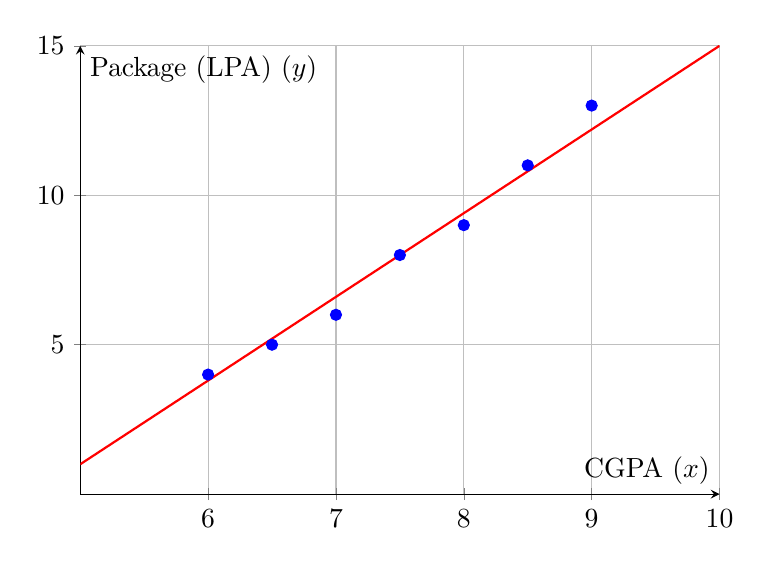
\begin{tikzpicture}
    \begin{axis}[
        xlabel={CGPA ($x$)},
        ylabel={Package (LPA) ($y$)},
        xmin=5, xmax=10,
        ymin=0, ymax=15,
        axis lines=middle,
        grid=major,
        width=0.8\textwidth,
        height=0.6\textwidth
    ]
    % Data Points
    \addplot[only marks, mark=*, color=blue] coordinates {
        (6, 4) (6.5, 5) (7, 6) (7.5, 8) (8, 9) (8.5, 11) (9, 13)
    };
    % Regression Line (Approx)
    \addplot[domain=5:10, color=red, thick] {2.8*x - 13};
    \end{axis}
\end{tikzpicture}
\caption{The concept of ``Best Fit Line''. The blue dots are actual students. The red line is our model.}
\label{fig:best_fit_intuition}
\end{figure}

The goal of Linear Regression is to find the \textbf{Best Fit Line}.
\begin{itemize}
    \item Imagine holding a straight stick over the scatter plot.
    \item You move the stick up, down, and rotate it until it passes \textit{as close as possible} to all the points.
    \item Effectively, you are trying to minimize the \textbf{total distance} (error) between the points and your stick.
\end{itemize}

\section{Mathematical Formulation}
Every straight line in the world can be written as:
\begin{equation}
    y = mx + c
\end{equation}
In Machine Learning, we often use slightly different notation:
\begin{equation}
    y = \beta_0 + \beta_1 x
\end{equation}
\begin{itemize}
    \item $y$: The Target (Dependent Variable).
    \item $x$: The Feature (Independent Variable).
    \item $\beta_1$ (Slope/Weight): Tells us \textit{how steeply} the Package rises with CGPA. If $\beta_1$ is high, a small increase in CGPA leads to a huge jump in salary.
    \item $\beta_0$ (Intercept/Bias): The baseline value. If CGPA is 0, what is the package? (Mathematically necessary, though practically CGPA isn't 0).
\end{itemize}


\section{Regression Evaluation Metrics}
Once we have drawn a line, how do we know how ``good'' it is?
Imagine you take an exam. The difference between your \textit{Expected Score} and \textit{Actual Score} is your ``Error''. We want to minimize this error across all students.

Let's say we have one prediction:
\begin{itemize}
    \item \textbf{Actual Package ($y$)}: 10 LPA
    \item \textbf{Predicted Package ($\hat{y}$)}: 12 LPA
    \item \textbf{Error}: $10 - 12 = -2$
\end{itemize}

\subsection{Mean Absolute Error (MAE)}
The simplest approach. We just take the absolute value of differences and average them.
\begin{equation}
    \text{MAE} = \frac{1}{n} \sum_{i=1}^{n} |y_i - \hat{y}_i|
\end{equation}
\textbf{Intuition}: On average, my prediction is off by $X$ LPA.
\begin{itemize}
    \item If errors are $[-2, +2, -5]$, Absolute errors are $[2, 2, 5]$. Average $= 3$.
    \item \textbf{Pros}: Robust to outliers.
    \item \textbf{Cons}: Not differentiable at 0 (V-shape), making it hard for some algorithms.
\end{itemize}

\subsection{Mean Squared Error (MSE)}
Here, we \textbf{square} the differences before averaging.
\begin{equation}
    \text{MSE} = \frac{1}{n} \sum_{i=1}^{n} (y_i - \hat{y}_i)^2
\end{equation}
\textbf{Why Square?}
\begin{enumerate}
    \item \textbf{Removes Negatives}: $(-2)^2 = 4$.
    \item \textbf{Punishes Big Errors}:
    \begin{itemize}
        \item Small Error (2) $\rightarrow$ Squared (4).
        \item Big Error (10) $\rightarrow$ Squared (100!).
    \end{itemize}
    \textit{The model gets terrified of making big mistakes.}
\end{enumerate}

\subsection{Root Mean Squared Error (RMSE)}
MSE is great, but the unit is wrong (LPA$^2$). We take the square root to bring it back to LPA.
\begin{equation}
    \text{RMSE} = \sqrt{\text{MSE}}
\end{equation}
This is the most popular metric. It penalizes large errors (like MSE) but is interpretable (like MAE).

\subsection{R-Squared ($R^2$ Score)}
RMSE gives us a number (e.g., ``Error is 2 LPA''), but is that good?
\begin{itemize}
    \item If the average package is 3 LPA, an error of 2 is terrible.
    \item If the average package is 50 LPA, an error of 2 is amazing.
\end{itemize}
$R^2$ gives a relative score between 0 and 1 (or 0\% to 100\%).
\begin{equation}
    R^2 = 1 - \frac{\text{Error of Our Line}}{\text{Error of Average Line}}
\end{equation}
\begin{itemize}
    \item \textbf{0.8 (80\%)}: Our model explains 80\% of the variation in salary. Good!
    \item \textbf{0.1 (10\%)}: Our model is useless.
\end{itemize}

\textbf{HOTS Question}: If your dataset has many outliers (e.g., one student getting 1 Crore package), which metric should you use: MAE or MSE?
\\ \textit{Answer: Use MAE. MSE would square that huge error, potentially forcing the line to shift drastically just to accommodate that one outlier.}


\section{Multiple Linear Regression}
When we have multiple input features (e.g., CGPA, Projects, Internships), the equation becomes a hyperplane:
\begin{equation}
    y = \beta_0 + \beta_1 x_1 + \beta_2 x_2 + \dots + \beta_n x_n
\end{equation}
Or in vector notation:
\begin{equation}
    Y = X\beta + \epsilon
\end{equation}

\section{Gradient Descent}
We have defined the error (MSE). Now, how do we find the line ($m$ and $c$) that gives the \textbf{Minimum Error}? We use an algorithm called \textbf{Gradient Descent}.

\subsection{Intuition: The Blindfolded Hiker}
Imagine you are standing on top of a mountain range. It is night, and there is thick fog. You are blindfolded. Your goal is to reach the deepest valley (the lowest point) where a village is located.

\begin{itemize}
    \item \textbf{Problem}: You cannot see the village.
    \item \textbf{Solution}: You feel the ground with your feet.
    \item \textbf{Strategy}:
    \begin{enumerate}
        \item If the ground slopes \textbf{down} towards the right, you take a step to the right.
        \item If the ground slopes \textbf{down} towards the left, you take a step to the left.
        \item You take small steps (Baby Steps) to avoid falling off a cliff.
        \item You repeat this until the ground feels flat (slope is 0). You have reached the valley!
    \end{enumerate}
\end{itemize}

In this analogy:
\begin{itemize}
    \item **Mountain Height**: The Loss (Error). High mountain = High Error.
    \item **Your Position**: The current values of weights ($m, c$).
    \item **Step Size**: The \textbf{Learning Rate} ($\alpha$ or $\eta$).
\end{itemize}

\subsection{Visualizing the Landscape}
\begin{figure}[htbp]
\centering
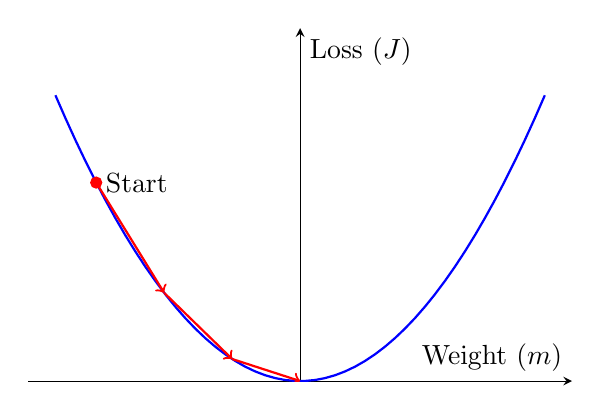
\begin{tikzpicture}
    \begin{axis}[
        xlabel={Weight ($m$)},
        ylabel={Loss ($J$)},
        xmin=-2, xmax=2,
        ymin=0, ymax=4,
        axis lines=middle,
        width=0.7\textwidth,
        height=0.5\textwidth,
        xtick=\empty, ytick=\empty
    ]
    % Loss Function Parabola
    \addplot[domain=-1.8:1.8, color=blue, thick, samples=50] {x^2};
    
    % Ball at step 1
    \addplot[only marks, mark=*, color=red] coordinates {(-1.5, 2.25)};
    \node[right] at (axis cs:-1.5, 2.25) {Start};
    
    % Arrow indicating movement
    \draw[->, thick, red] (axis cs:-1.5, 2.25) -- (axis cs:-1.0, 1.0);
    \draw[->, thick, red] (axis cs:-1.0, 1.0) -- (axis cs:-0.5, 0.25);
    \draw[->, thick, red] (axis cs:-0.5, 0.25) -- (axis cs:0, 0);
    
    \node[below] at (axis cs:0, 0) {Global Minima};
    \end{axis}
\end{tikzpicture}
\caption{Gradient Descent: A ball rolling down the Loss Curve to find the minimum.}
\label{fig:gd_analogy}
\end{figure}

\subsection{The Math (Update Rule)}
We update our weights ($m$) using the gradient (slope):
\begin{equation}
    m_{new} = m_{old} - \eta \times \text{Slope}
\end{equation}
\begin{itemize}
    \item \textbf{Minus Sign}: Because we want to go \textit{against} the slope (Downhill).
    \item $\eta$ (\textbf{Learning Rate}): Controls how big our step is.
\end{itemize}

\textbf{HOTS Question}: What happens if your Learning Rate ($\eta$) is too high?
\\ \textit{Answer: You might take a giant step and jump across the valley to the other side, possibly climbing higher up! The model will diverge and never find the solution.}


\section{Types of Gradient Descent}
Based on how much data is used to calculate the gradient in one step, there are three main types:

\subsection{Batch Gradient Descent}
\begin{itemize}
    \item \textbf{Method}: Uses the \textbf{entire dataset} to calculate the gradient and update weights once.
    \item \textbf{Pros}: Smooth convergence, stable error gradient.
    \item \textbf{Cons}: Very slow for large datasets; high memory usage.
\end{itemize}

\subsection{Stochastic Gradient Descent (SGD)}
\begin{itemize}
    \item \textbf{Method}: Uses a \textbf{single random data point} to calculate the gradient and update weights.
    \item \textbf{Pros}: Extremely fast iterations, uses little memory.
    \item \textbf{Cons}: Noisy convergence (zigzag path), might not settle clearly at global minima.
\end{itemize}

\subsection{Mini-Batch Gradient Descent}
\begin{itemize}
    \item \textbf{Method}: Uses a \textbf{small batch} of data points (e.g., 32 or 64) for one update.
    \item \textbf{Pros}: Best of both worlds—stable like Batch and fast like SGD. Standard choice in Deep Learning.
\end{itemize}

\begin{table}[htbp]
    \centering
    \caption{Comparison of Gradient Descent Types}
    \begin{tabular}{|l|l|l|l|}
    \hline
    \textbf{Feature} & \textbf{Batch GD} & \textbf{Stochastic GD} & \textbf{Mini-Batch GD} \\ \hline
    \textbf{Data per Step} & All ($n$) & One ($1$) & Batch ($k$) \\ \hline
    \textbf{Speed per Step} & Slow & Very Fast & Fast \\ \hline
    \textbf{Convergence} & Smooth & Noisy/Zigzag & Smoother than SGD \\ \hline
    \textbf{Memory} & High & Low & Moderate \\ \hline
    \end{tabular}
\end{table}

\section{Polynomial Regression}
What if the data relationships are non-linear? A straight line ($y=mx+c$) won't fit well.
Polynomial Regression allows us to fit curves by adding powers of the original features as new features.

Equation for degree 2:
\begin{equation}
    y = \beta_0 + \beta_1 x + \beta_2 x^2
\end{equation}
Although it fits a curve, it is still considered \textbf{Linear Regression} because it is linear in terms of \textbf{coefficients} ($\beta$).

\section{Implementation in Python}
Let's build a Linear Regression model from scratch using \texttt{scikit-learn}. We will use a simple dataset to predict a package based on CGPA.

\begin{lstlisting}[language=Python, caption=Linear Regression Step-by-Step]
import numpy as np
import pandas as pd
import matplotlib.pyplot as plt
from sklearn.model_selection import train_test_split
from sklearn.linear_model import LinearRegression
from sklearn.metrics import mean_absolute_error, mean_squared_error, r2_score

# Step 1: Create Dummy Data
# 100 students with CGPA between 5 and 10
X = np.random.uniform(5, 10, 100).reshape(-1, 1) 
# Package roughly follows: 2 * CGPA - 5 (plus some random noise)
y = 2 * X - 5 + np.random.normal(0, 1, (100, 1))

# Step 2: Split Data (80% for Training, 20% for Testing)
# Why? We must evaluate the model on Unseen Data to check for overfitting.
X_train, X_test, y_train, y_test = train_test_split(X, y, test_size=0.2, random_state=42)

# Step 3: Train the Model
model = LinearRegression()
model.fit(X_train, y_train) # The model learns 'm' and 'c' here

# Step 4: Make Predictions
y_pred = model.predict(X_test)

# Step 5: Evaluate
print("MAE:", mean_absolute_error(y_test, y_pred))
print("RMSE:", np.sqrt(mean_squared_error(y_test, y_pred)))
print("R2 Score:", r2_score(y_test, y_pred))

# Step 6: Visualizing the Result
plt.scatter(X, y, color='blue', label='Actual Data') # Plot all points
plt.plot(X_test, y_pred, color='red', label='Prediction Line') # Plot the line
plt.xlabel('CGPA')
plt.ylabel('Package')
plt.legend()
plt.show()
\end{lstlisting}

\section{Key Takeaways}
\begin{itemize}
    \item \textbf{Linear Assumption}: We assume the data follows a straight line ($y = mx + c$).
    \item \textbf{Best Fit}: The best line is the one that minimizes the \textbf{Squared Error} (MSE) between actual and predicted points.
    \item \textbf{Gradient Descent}: The algorithm used to find the best line by iteratively walking down the error mountain.
    \item \textbf{Metrics}: We use RMSE to measure error in the same unit as the target, and $R^2$ to understand how much variance we captured (0 to 1).
\end{itemize}


\section{Bias-Variance Tradeoff}
This is a central problem in supervised learning. Ideally, we want a model that accurately captures the regularities in its training data, but also generalizes well to unseen data.

\subsection{Definitions}
\begin{itemize}
    \item \textbf{Bias}: Error due to overly simplistic assumptions in the learning algorithm. High bias can cause an algorithm to miss the relevant relations between features and target outputs (\textbf{Underfitting}).
    \item \textbf{Variance}: Error due to too much complexity in the learning algorithm. High variance causes overfitting: modeling the random noise in the training data (\textbf{Overfitting}).
\end{itemize}

\subsection{The Tradeoff}
\begin{itemize}
    \item \textbf{High Bias (Underfitting)}: Model is too simple (e.g., straight line for curved data). High error on training and test data.
    \item \textbf{High Variance (Overfitting)}: Model is too complex (e.g., high-degree polynomial). Low error on training data, high error on test data.
    \item \textbf{Goal}: Find the sweet spot where both bias and variance are low (Total Error is minimized).
\end{itemize}

\section{Regularization}
Regularization is a technique used to prevent \textbf{overfitting} by adding a penalty term to the Loss Function. It discourages complex models (large coefficients).

\subsection{Ridge Regression (L2 Regularization)}
Adds specific penalty equivalent to sum of the squares of the magnitude of coefficients.
\begin{equation}
    J = \text{MSE} + \lambda \sum_{i=1}^{n} \beta_i^2
\end{equation}
\begin{itemize}
    \item $\lambda$ (Lambda): Regularization strength.
    \item Shrinks coefficients towards zero but rarely makes them exactly zero.
    \item Useful when \textbf{multicollinearity} exists.
\end{itemize}

\subsection{Lasso Regression (L1 Regularization)}
Adds a penalty equivalent to sum of the absolute value of coefficients.
\begin{equation}
    J = \text{MSE} + \lambda \sum_{i=1}^{n} |\beta_i|
\end{equation}
\begin{itemize}
    \item Can shrink coefficients \textbf{exactly to zero}.
    \item Useful for \textbf{Feature Selection} (removes useless features).
\end{itemize}

\subsection{Elastic Net}
Combines both L1 and L2 penalties.
\begin{equation}
    J = \text{MSE} + \lambda_1 \sum |\beta_i| + \lambda_2 \sum \beta_i^2
\end{equation}
Useful when there are multiple features correlated with each other. Lasso is likely to pick one of these at random, while Elastic-net is likely to pick both.


